\icode{O-MD-CA-L3-261113-003}
如图所示，一{\kaishu\color{orange}足够长}的水平传送带以恒定的速度\(v_0\)向右传动。物体以\(v\)的速度冲传送带右端，传送带与零件间的动摩擦因数为 \(\mu\)。作出\(v - t\)图像。

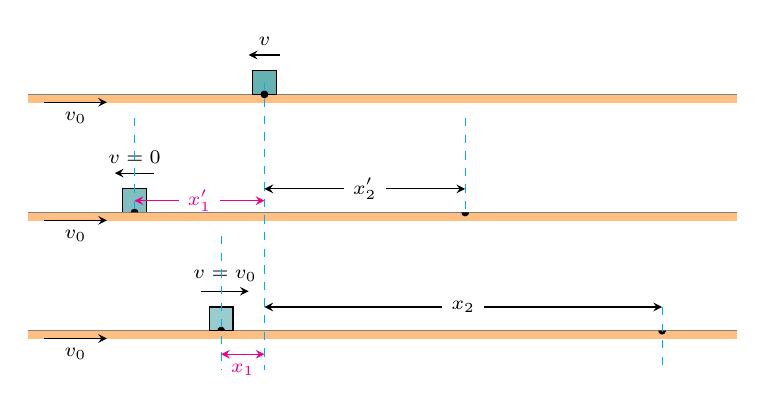
\begin{tikzpicture}[>=stealth,font=\scriptsize]
	\begin{scope}
		\draw[fill=orange!50,draw=orange!50] (-3,0) rectangle(6,-.1);
		\draw[gray] (-3,0)--(6,0);
		\draw[fill=teal!60] (-.15,0) rectangle(.15,.3);
		\fill (0,0) circle(.05);
		\draw[->] (.2,.5)--node[above]{\(v\)}(-.2,.5);
		\draw[->] (-2.8,-.1)--node[below]{\(v_0\)}(-2,-.1);
	\end{scope}
	\begin{scope}[yshift=-1.5cm]
        \draw[fill=teal!50] (-1.8,0) rectangle(-1.5,.3);
        \draw[<->,thin,magenta] (-1.65,.15)--node[fill=white]{\(x_1^{\prime}\)}(0,.15);
		\draw[fill=orange!50,draw=orange!50] (-3,0) rectangle(6,-.1);
		\draw[gray] (-3,0)--(6,0);
		\fill (-1.7,0) arc(180:0:.05)--cycle;
		\fill (2.5,0) arc(-180:0:.05)--cycle;
		\draw[->] (-1.4,.5)--node[above]{\(v = 0\)}(-1.9,.5);
		\draw[->] (-2.8,-.1)--node[below]{\(v_0\)}(-2,-.1);
	\end{scope}
	\begin{scope}[yshift=-3cm]
		\draw[fill=orange!50,draw=orange!50] (-3,0) rectangle(6,-.1);
		\draw[gray] (-3,0)--(6,0);
		\draw[fill=teal!40] (-.7,0) rectangle(-.4,.3);
		\fill (-.6,0) arc(180:0:.05)--cycle;
		\fill (5,0) arc(-180:0:.05)--cycle;
		\draw[->] (-.8,.5)--node[above]{\(v = v_0\)}(-.2,.5);
		\draw[->] (-2.8,-.1)--node[below]{\(v_0\)}(-2,-.1);
	\end{scope}
	\draw[dashed,cyan] (0,.15)--(0,-3.5) (-1.65,-.3)--(-1.65,-1.5) (-.55,-1.8)--(-.55,-3.5) (2.55,-.3)--(2.55,-1.5) (5.05,-2.7)--(5.05,-3.5);
	\draw[<->,thin] (0,-1.2)--node[fill=white]{\(x_2^{\prime}\)}(2.55,-1.2);
	\draw[<->,thin] (0,-2.7)--node[fill=white]{\(x_2\)}(5.05,-2.7);
	\draw[<->,thin,magenta] (-.55,-3.3)--node[below]{\(x_1\)}(0,-3.3);
\end{tikzpicture}
\begin{tikzpicture}[>=stealth,font=\scriptsize]
	\begin{scope}
		\draw[->,blue] (0,0)node[left]{\(O\)}--(4,0)node[right]{\(t\)};
		\draw[->,blue] (0,-2)--(0,2)node[right]{\(v\)};
	\end{scope}
\end{tikzpicture}